\documentclass[a4paper,12pt]{article}
\usepackage{styles/iplouccfg}
\usepackage{styles/zhfontcfg}
\usepackage{styles/iplouclistings}


\title{视网膜图像配准} %标题
\author{孙雪}  %作者
\date{2013年08月12日} %日期,不加默认为当前日期

\begin{document}

\maketitle
\tableofcontents %目录
\newpage
\section{绪论}

\subsection{图像配准的相关理论}

\subsubsection{图像配准的基本概念}

在拍摄同一场景的图像时,由于拍摄的时间、角度、光线、温度、大气折射等因素,拍摄出的图像可能会造成一定程度的旋转、不同比例的缩放、不同的灰度属性等问题。图像匹配是对同一场景在不同条件下得到的两幅或多幅图像进行对准、叠加的过程。图像匹配的目的就是寻找一种变换,将一幅图像映射到另一幅图像,使得两幅图像的相似程度达到最大。

图像配准的数学描述可以定义为参考图像和待配准图像之间的空间变换及灰度变换。如果将图像表示为一个二维矩阵,$I_1(x,y)$、$I_2(x,y)$分别表示两幅图像在点$(x,y)$处的灰度值,那么图像$I_1$、$I_2$的配准关系可用式(\ref{eq:1})表示。
\begin{equation} 
\label{eq:1}
I_2(x,y)=g(I_1(f(x,y)))
\end{equation}

其中,$I_1$和$I_2$表示两幅待匹配图像表示的二维矩阵,$I_1(x,y)$、$I_2(x,y)$表示两幅图像在$(x,y)$处的灰度值,$g$是一维灰度变换,$f$表示一个二维坐标变换。

配准的过程就是寻找最优的空间变换和灰度变换参数,使图像间达到匹配。实际应用中,我们常常关心的是坐标变换,于是,配准关系可以简化为式(\ref{eq:2})。
\begin{equation} 
\label{eq:2}
I_2(x,y)=I_1(f_x(x,y),f_y(x,y))
\end{equation}

\subsubsection{图像配准的一般流程}

图像配准一般都会包括四个步骤:特征检测、特征匹配、变换模型参数估计、重采样和插值。

\begin{enumerate}
\item 特征检测:特征检测是指人工或自动地检测出图像的显著特征和突出的目标。利用这些关键点就可以估计出两幅待配准图像之间的空间几何变换关系。特征检测一般包括两个步骤,特征提取和特征描述。把特征提取出来,并用一些特征描述算子来表示特征,以便进行特征匹配。
\item 特征匹配:特征匹配的目的是找到参考图像和待配准图像的特征之间的对应关系。通过对特征检测得到的特征描述算子进行相似性度量等操作来得到最佳的匹配特征及他们之间的对应关系。
\item 变换模型参数估计:空间变换模型参数估计的目的是要估计出连接参考图像和待配准图像的映射函数的类型及参数。其中映射函数的参数通过特征匹配来计算得到。
\item 重采样和插值:重采样和插值指的是待配准图像通过映射函数进行空间几何变换。其中图像中非整数坐标的灰度值需要通过恰当的插值技术计算。
\end{enumerate}
\subsection{图像配准技术的国内外研究现状}

现有的图像配准算法大致可分为基于灰度和基于特征的方法两类。基于灰度的配准方法直接利用图像的灰度值来确定待配准图像之间的空间几何变换关系。它没有特征检测的步骤,在特征匹配阶段,利用固定大小的窗口来进行匹配估计,因此计算简单,易于实现。但在图像中存在较多噪声或两幅待配准图像中的重叠部分较少的情况下,配准效果不太理想。基于特征的方法将对整个图像非分析转化为对图像特征的分析,大大减小了图像处理过程中的运算量,对灰度变化、图像变形也有较好的适应能力。

\subsubsection{基于灰度的图像配准}

基于灰度的图像配准方法是最早发展起来的,利用图像本身的灰度统计信息来度量图像的相似程度,采用一定的搜索算法得到相似度最大的变换形式,来达到配准图像的目的。

基于灰度的图像配准方法主要有三类:相关算法、基于傅里叶变换的相位相关方法、互信息法。相关法计算待配准图像间的相关系数、方差等值,来使相关性达到最大,从而实现配准。Barnea\cite{8:article}等提出了一种序贯检测算法,有计算量小、运算速度快的特点,但必须是在两幅待配准图像之间有接近灰度的前提下。Pratt\cite{9:article}等针对存在噪声的图像,利用滤波的方法对图像进行预处理来提高配准的性能。Roche\cite{10:article}等采用了相关比率法解决了经典的互相关法不能处理不同灰度尤其是不同传感器图像的缺点。

基于傅里叶变换的相位相关方法通过计算两幅待配准图像的互功率普的相位来得到它们的平移参数,这样就把空域上的相关运算转化到了频率上的复数乘法运算。Castro等在经典的相位相关法的基础上加入了旋转变换\cite{11:article}。Chen\cite{12:article}及Reddy\cite{13:article}等将结合了相位相关和傅里叶梅林变换的方法应用到图像配准和目标识别当中,解决了图像之间存在尺度、旋转和平移变化的情况。

互信息法在遥感图像配准和医学图像配准领域受到广泛关注,因为互信息法不需要预处理及图像分割,配准精度相对较高。原理是通过将两幅待配准图像看成是两个随机变量,当两幅图像达到空间上的一致时,互信息也达到最大。最早利用互信息法进行图像配准包括Viola等,他们利用互信息法完成了医学核磁共振图像的配准、三维目标模型和真实世界图像的配准\cite{14:article}。Studholme等提出了归一化互信息配准,降低了传统互信息计算中对于重叠区域大小的敏感度\cite{15:article}。Pluim等采用由粗到细的分层次对互信息图像配准进行了加速\cite{16:article}。今年来,有学者提出在互信息配准中加入图像的梯度、共生矩阵、特征点的等信息,使得互信息配准的精度和鲁棒性得到增强。

\subsubsection{基于特征的图像配准}

基于特征的图像配准主要利用图像的区域、边缘、轮廓、特征点等图像上显著的特征,根据这些特征来估算图像间的变换模型,这种算法大大减少了图像的信息。

图像的区域特征主要包括建筑物、湖泊、森林等,主要通过图像分割的方法进行检测。图像分割的准确性很大程度上影响了配准结果的好坏。Goshtasby将区域的重心作为关键点来进行图像配准\cite{17:phdthesis},Ton等将片状区域的质心作为关键点进行图像配准\cite{18:article}。

图像的边缘是指图像中在某个方向上灰度变化剧烈而与这个方向正交的方向上灰度变换缓慢的一系列像素。首先应采用边缘检测算法将边缘提取出来。Mount等将提取的边缘点作为图像的特征点,利用Hausdorff距离作为相似度度量准则对特征进行了匹配\cite{19:article}。

基于轮廓的图像配准首先提取图像中的轮廓特征,然后对轮廓进行匹配从而得到图像之间的几何变换关系。Tham等对检测出的轮廓特征用链码的形式表示,并通过链码间接的进行轮廓匹配\cite{20:article}。Yuan等将金字塔策略应用到基于轮廓的配准方法中\cite{21:article}。

图像的特征点一般是图像在各个方向灰度变换都较大的点,例如图像中的拐点,交叉点,区域的重心等等。1997年,Moravec提出了从灰度图像中提取角点的算法\cite{22:proceedings},Harris等对Moravec算子进行了改进,对图像的旋转变换具有不变性\cite{23:proceedings}。后来一些学者纷纷提出把Harris算法与互信息及相位相关方法相结合来进行图像配准,很大程度上促进了图像配准的发展。Lowe提出尺度不变特征检测的方法,该方法检测出的特征点在图像尺度变换、旋转、光照和视角变化的条件下都具有很好的不变性\cite{24:proceedings},2004年又提出SIFT算法,将特征点检测、描述及匹配作为一个统一的过程,对计算机视觉研究影响深远\cite{25:article}。Bay等提出了SURF算法,大大提高了SIFT的计算速度\cite{26:proceedings}。

\subsection{视网膜图像配准的发展}

视网膜图像配准是辅助眼科医生诊断各种眼类疾病的关键。视网膜图像中含有宝贵的局部视网膜信息,是由不同时间和不同角度拍摄得来的。准确的配准有助于眼科医生进行更好的诊断并制定治疗计划。近几年,大量的图像配准算法已经提出。

Matsopoulos等基于视网膜分割图像的强度差异,采用模拟退火和遗传算法优化目标函数\cite{5:article}。Ritter等人利用互信息与模拟退火相结合来对准立体视网膜图像及不同时间采集的视网膜图像\cite{6:article}。此外,基于金字塔采样的退火搜索技术减少了运行时间,提高了效率。Skokan等利用互信息作为匹配标准,但主要的缺点就是计算量大\cite{7:article}。基于灰度的图像配准需要用整个图像的信息来计算图像的相似性度量,计算比较复杂。如果待配准图像的重叠区域不足够大,基于灰度的配准方法可能会导致大的偏差。

基于特征的方法首先要提取视网膜图像的特征,比如血管分叉点、整个血管、视盘、由点式探测器提取的特征点等。用特征对应的目标函数求最好的变换参数。目前,大多数基于特征的方法是以血管作为特征的。Chan等人提取整个血管树用来进行图像配准。Zana等人利用分叉点的分支角度作为特征来进行匹配\cite{1:article}。由于一个分叉点可能在另一幅图像上有几个与之相对应,Can等人提出分层方法来解决这个问题\cite{2:article}。Stewart等人利用血管分叉点作为关键点,采用双引导迭代最近点算法(Dual-Bootstrap ICP)扩大区域和细化变换模型\cite{3:article}。一种无监督的自组织映射方法对于多模态的匹配有较好的效果\cite{4:article}。
基于特征的方法在待配准图像重叠区域较小的情况下能更快更有效的进行配准。

\section{基于分叉结构的视网膜图像配准}

\subsection{理论}

传统的点匹配方法很大程度上依赖于单分叉点的分支角度。一幅图像上的一个分支角度可能与另一幅图像上几个分支角度值相似,这样以单分叉点的分支角度作为特征会导致匹配对应关系的增多,从而降低配准精度。基于分叉结构的视网膜图像配准是以一个主分叉点及与它相邻的三个分叉点作为一个结构特征来进行匹配,这样就会大大减小一对多匹配的可能性。

\subsubsection{分支结构}

\begin{figure}[!htb] %插图
\centering
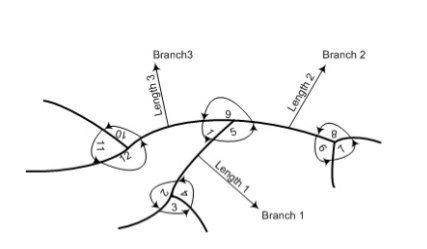
\includegraphics[width=0.8\textwidth]{Bifucation.png}
\caption{分叉结构}
\label{fig:1}
\end{figure}

如图\ref{fig:1}所示,一个分叉结构是由一个主分叉和三个相邻的分叉组成。主分叉与三个相邻分叉的距离为$Length1,Length2,Length3$,它的分叉角度为$1,5,9$。以分叉结构来作为特征进行图像匹配。用一个特征向量来描述分叉结构:
\begin{equation} 
\label{eq:3}
\boldsymbol{x}=\{lengths,angles\}=[l_1,l_2,l_3,\alpha_1,\alpha_2,\alpha_3,\alpha_4,\alpha_5,\alpha_6,\alpha_7,\alpha_8,\alpha_9,\alpha_{10},\alpha_{11},\alpha_{12}]
\end{equation}

其中,$l_i$和$\alpha_i$分别代表归一化的长度和角度:
\begin{equation} 
\label{eq:4}
\begin{array}{l}
l_i=i-th\quad branch\quad length/sum\{length 1,length 2,length 3\}\\
\alpha_i=i-th\quad branch\quad angle\quad in\quad degree/360^{\circ}
\end{array}
\end{equation}

需要注意的是,$x$应该按分支的长度进行排列,第一个元素代表最长的分支长度,这样就能保证特征向量对于平移和缩放是不变的。

\subsubsection{相似性度量}

特征匹配的过程就是寻找最相似的分支结构对的过程。如果$X$和$Y$分别代表两幅图像中的特征组,包含的分支结构的数量为$M_1$和$M_2$,则分叉结构对的相似性度量$s_{i,j}$为:

\begin{equation} 
\label{eq:5}
s_{i,j}=d(\boldsymbol{x}_i,\boldsymbol{y}_i)
\end{equation}

其中$\boldsymbol{x}_i$和$\boldsymbol{y}_i$分别表示两幅图像中第$i$个和第$j$个分支结构的特征向量。$d()$表示特征向量之间的距离测度。

\subsubsection{确认匹配}

与单一分叉点的三个角度作为特征向量相比,以分叉结构作为特征向量包含了长度和角度的信息。这一功能有利于减少匹配过程中的一对多的情况,如图\ref{fig:2}所示。(a)表示单一分叉点的匹配,(b)表示以分叉结构作为特征的匹配。
\begin{figure}[!htb] %插图
\centering
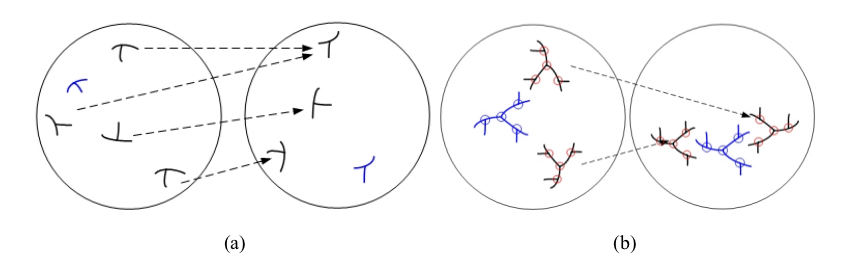
\includegraphics[width=1.0\textwidth]{matching.png}
\caption{两种特征的匹配对比}
\label{fig:2}
\end{figure}

虽然以分叉结构作为特征来进行匹配能大大提高配准的准确度,但是难免会出现一些错误匹配的情况。利用特征间的空间关系进行特征分解的方法可以验证和纠正初期的对应关系。

众所周知,线性变换对于对应点的最低要求是两对,仿射是三对。因此,一个匹配的分叉结构足够估计变换模型的参数,因为它提供了四对对应点。相应的细化和变换估计可以通过式(\ref{eq:6})同时实现:
\begin{equation} 
\label{eq:6}
e_{(pq,mn)}=d\big(M(\boldsymbol{x}_p,\boldsymbol{y}_q),M(\boldsymbol{x}_m,\boldsymbol{y}_n)\big)
\end{equation}

这里,$M(\boldsymbol{x}_p,\boldsymbol{y}_q)$和$M(\boldsymbol{x}_m,\boldsymbol{y}_n)$分别是匹配对$\boldsymbol{x}_p$和$\boldsymbol{y}_q$,$\boldsymbol{x}_m$和$\boldsymbol{y}_n$的变换模型估计。

在确认匹配这个过程中,分叉结构对必须具有良好相似性度量\ref{eq:5}。通过这种方式,移除了杂乱的对应关系,来得到良好的分叉结构对。这写分叉结构对可以用来估计变换模型。



\subsection{流程(程序部分)}

\begin{figure}
\centering
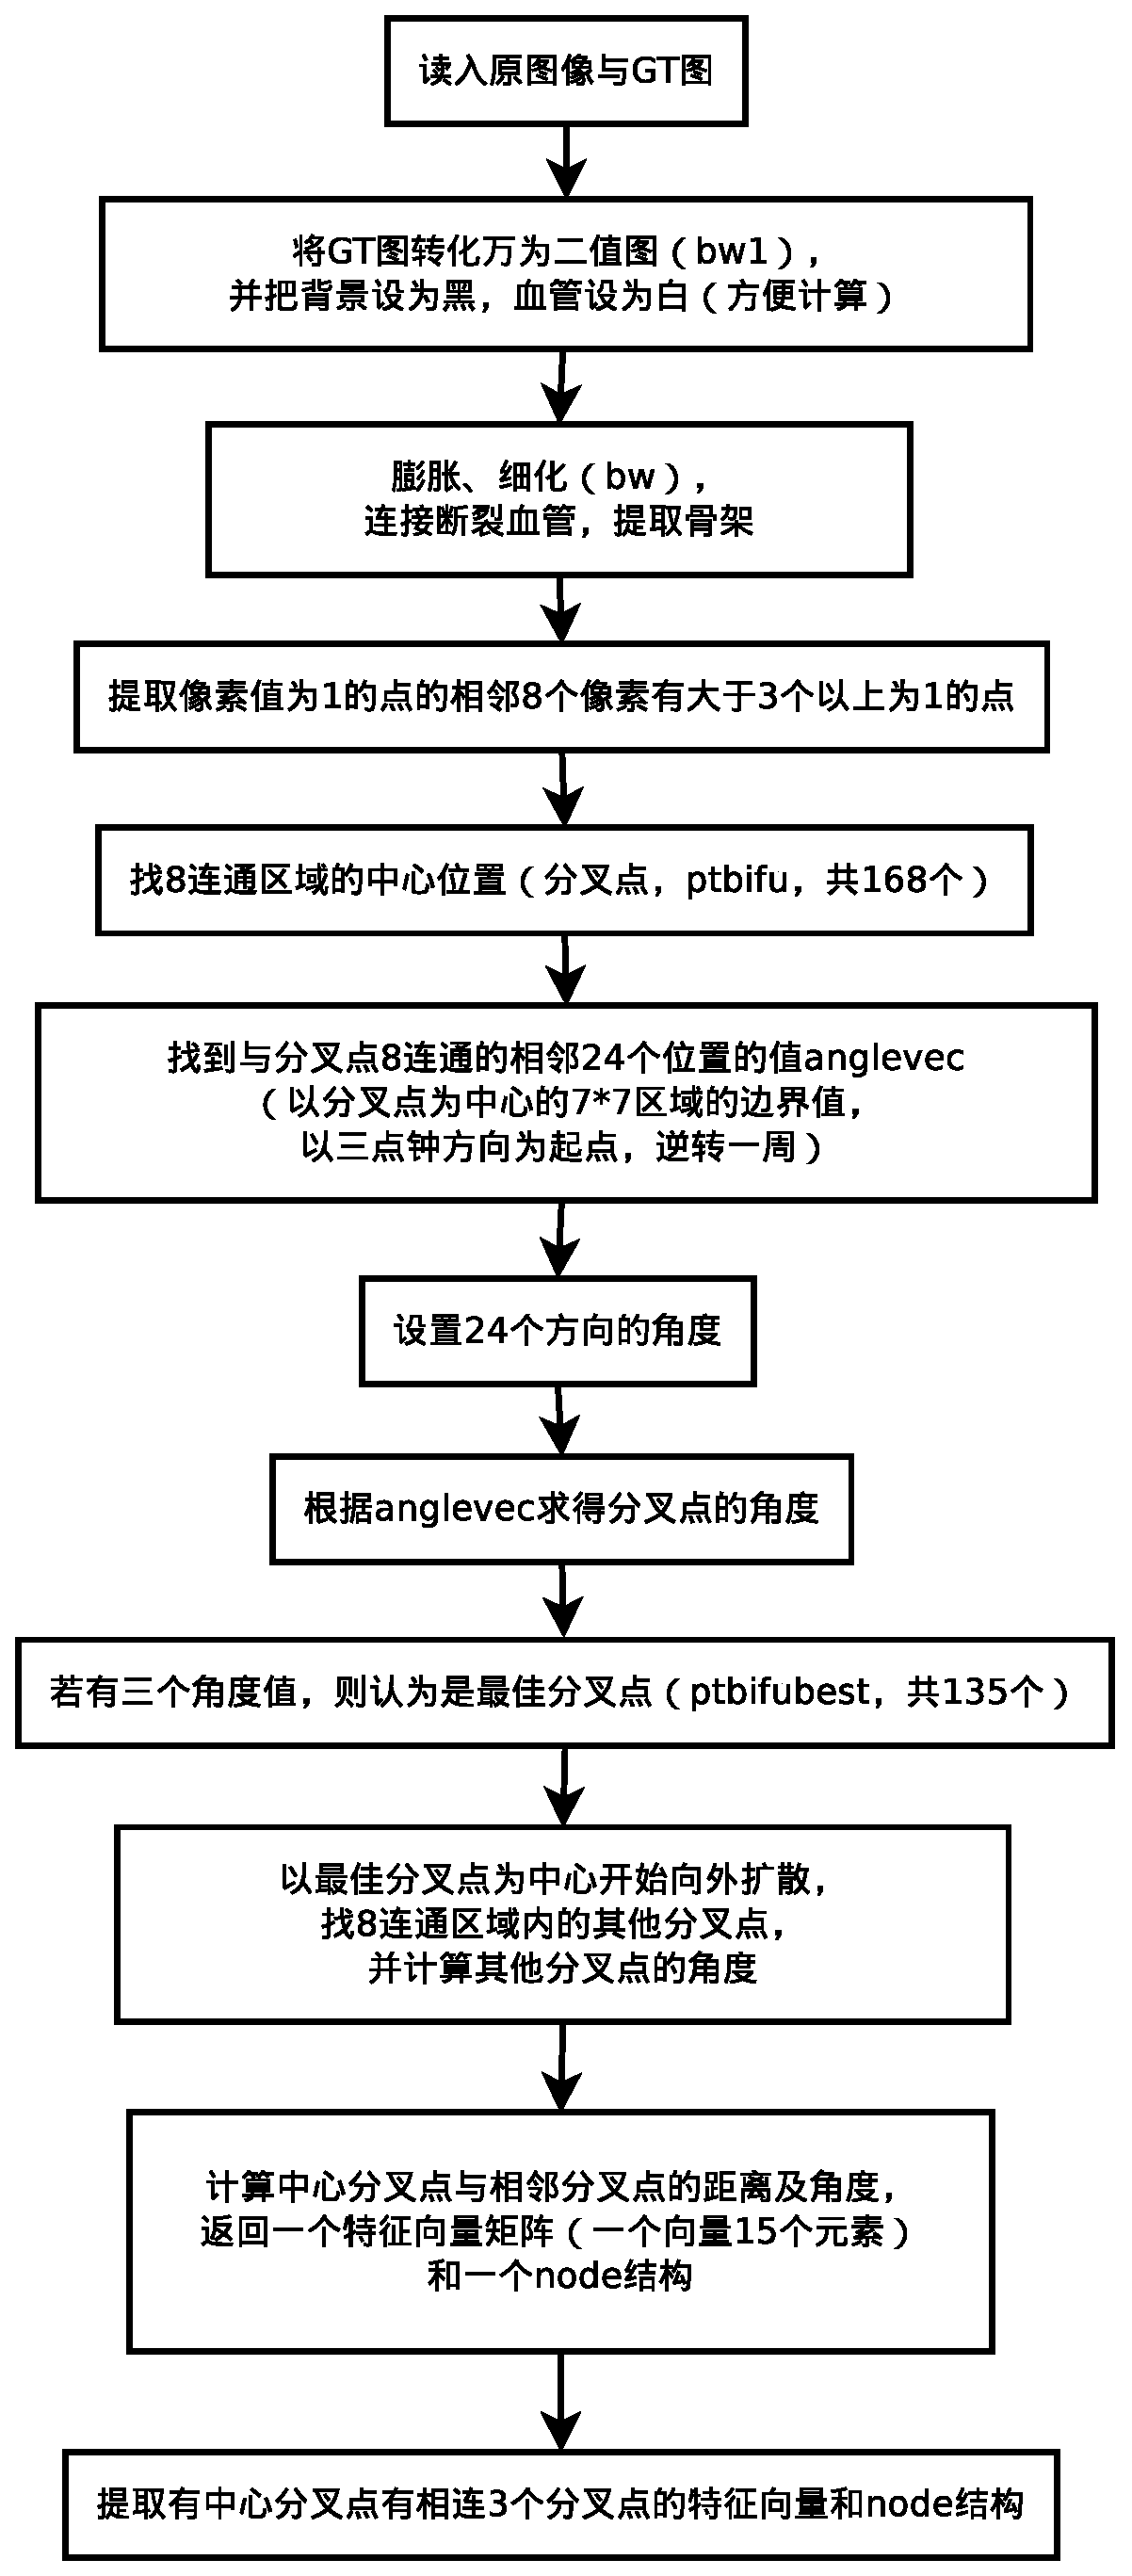
\includegraphics[width=0.6\textwidth]{feature-registration}
\caption{特征向量的产生}
\label{fig:3}
\end{figure}

\begin{figure}
\centering
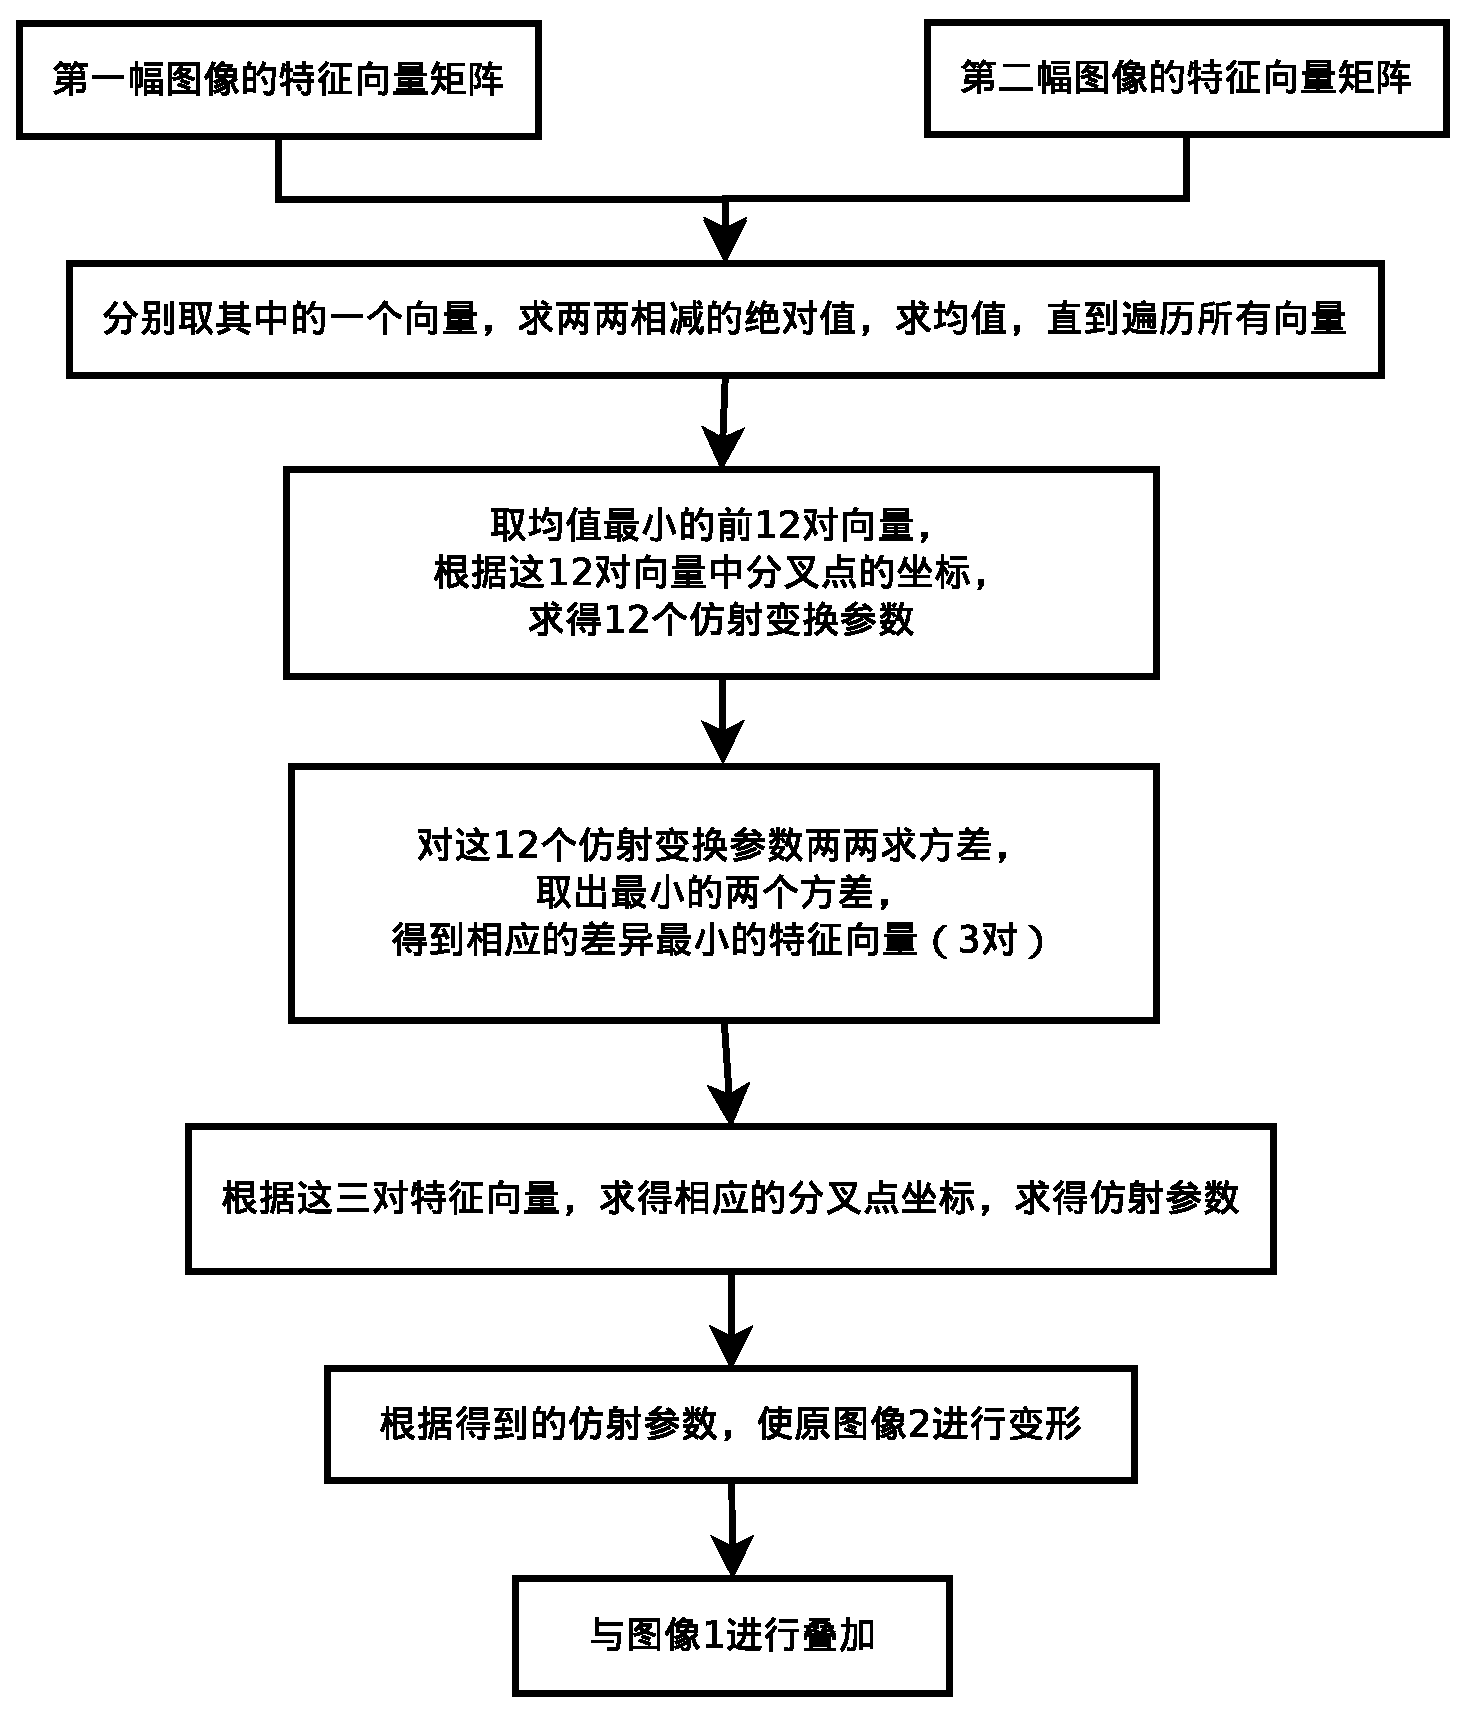
\includegraphics[width=0.8\textwidth]{registration.eps}
\caption{匹配与变形}
\label{fig:4}
\end{figure}






\newpage

% references
\bibliographystyle{plain}
\bibliography{Retinal_image_registration} %参考文献

\end{document}
